% Created by tikzDevice version 0.12.6 on 2024-02-25 11:57:34
% !TEX encoding = UTF-8 Unicode
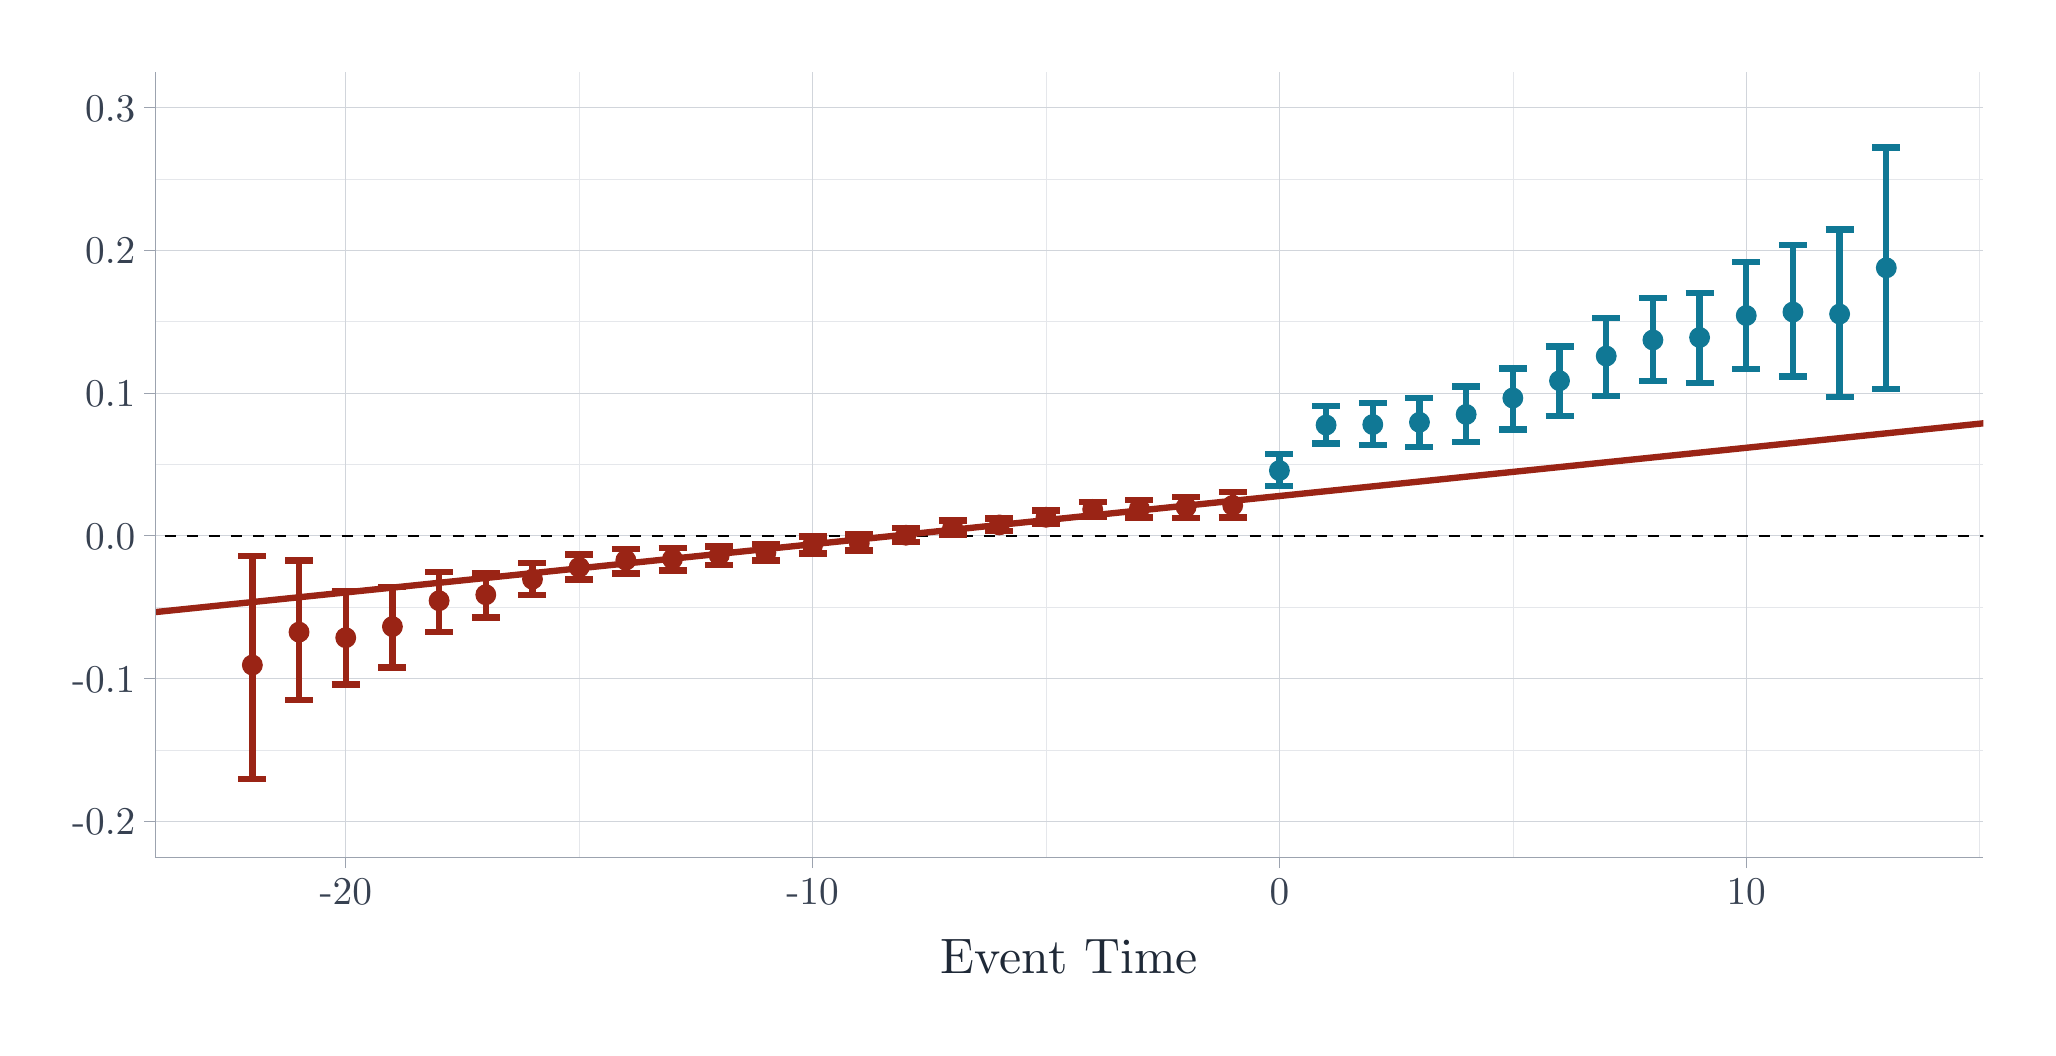
\begin{tikzpicture}[x=1pt,y=1pt]
\definecolor{fillColor}{RGB}{255,255,255}
\path[use as bounding box,fill=fillColor] (0,0) rectangle (722.70,361.35);
\begin{scope}
\path[clip] (  0.00,  0.00) rectangle (722.70,361.35);
\definecolor{drawColor}{RGB}{255,255,255}

\path[draw=drawColor,line width= 0.8pt,line join=round,line cap=round,fill=fillColor] (  0.00,  0.00) rectangle (722.70,361.35);
\end{scope}
\begin{scope}
\path[clip] ( 46.10, 61.65) rectangle (706.70,345.35);
\definecolor{drawColor}{RGB}{255,255,255}
\definecolor{fillColor}{RGB}{255,255,255}

\path[draw=drawColor,line width= 0.8pt,line join=round,line cap=round,fill=fillColor] ( 46.10, 61.65) rectangle (706.70,345.35);
\definecolor{drawColor}{RGB}{229,231,235}

\path[draw=drawColor,line width= 0.2pt,line join=round] ( 46.10,100.34) --
	(706.70,100.34);

\path[draw=drawColor,line width= 0.2pt,line join=round] ( 46.10,151.92) --
	(706.70,151.92);

\path[draw=drawColor,line width= 0.2pt,line join=round] ( 46.10,203.50) --
	(706.70,203.50);

\path[draw=drawColor,line width= 0.2pt,line join=round] ( 46.10,255.08) --
	(706.70,255.08);

\path[draw=drawColor,line width= 0.2pt,line join=round] ( 46.10,306.66) --
	(706.70,306.66);

\path[draw=drawColor,line width= 0.2pt,line join=round] (199.28, 61.65) --
	(199.28,345.35);

\path[draw=drawColor,line width= 0.2pt,line join=round] (367.97, 61.65) --
	(367.97,345.35);

\path[draw=drawColor,line width= 0.2pt,line join=round] (536.66, 61.65) --
	(536.66,345.35);

\path[draw=drawColor,line width= 0.2pt,line join=round] (705.35, 61.65) --
	(705.35,345.35);
\definecolor{drawColor}{RGB}{209,213,219}

\path[draw=drawColor,line width= 0.4pt,line join=round] ( 46.10, 74.55) --
	(706.70, 74.55);

\path[draw=drawColor,line width= 0.4pt,line join=round] ( 46.10,126.13) --
	(706.70,126.13);

\path[draw=drawColor,line width= 0.4pt,line join=round] ( 46.10,177.71) --
	(706.70,177.71);

\path[draw=drawColor,line width= 0.4pt,line join=round] ( 46.10,229.29) --
	(706.70,229.29);

\path[draw=drawColor,line width= 0.4pt,line join=round] ( 46.10,280.87) --
	(706.70,280.87);

\path[draw=drawColor,line width= 0.4pt,line join=round] ( 46.10,332.45) --
	(706.70,332.45);

\path[draw=drawColor,line width= 0.4pt,line join=round] (114.93, 61.65) --
	(114.93,345.35);

\path[draw=drawColor,line width= 0.4pt,line join=round] (283.62, 61.65) --
	(283.62,345.35);

\path[draw=drawColor,line width= 0.4pt,line join=round] (452.31, 61.65) --
	(452.31,345.35);

\path[draw=drawColor,line width= 0.4pt,line join=round] (621.00, 61.65) --
	(621.00,345.35);
\definecolor{drawColor}{RGB}{0,0,0}

\path[draw=drawColor,line width= 0.9pt,dash pattern=on 4pt off 4pt ,line join=round] (-614.49,177.71) -- (1367.30,177.71);
\definecolor{drawColor}{RGB}{154,36,21}

\path[draw=drawColor,line width= 2.3pt,line join=round] (-614.49, 81.94) -- (1367.30,286.61);
\definecolor{fillColor}{RGB}{154,36,21}

\path[draw=drawColor,line width= 0.4pt,line join=round,line cap=round,fill=fillColor] ( 81.19,131.04) circle (  3.57);

\path[draw=drawColor,line width= 0.4pt,line join=round,line cap=round,fill=fillColor] ( 98.06,142.93) circle (  3.57);

\path[draw=drawColor,line width= 0.4pt,line join=round,line cap=round,fill=fillColor] (114.93,140.92) circle (  3.57);

\path[draw=drawColor,line width= 0.4pt,line join=round,line cap=round,fill=fillColor] (131.80,144.92) circle (  3.57);

\path[draw=drawColor,line width= 0.4pt,line join=round,line cap=round,fill=fillColor] (148.67,154.27) circle (  3.57);

\path[draw=drawColor,line width= 0.4pt,line join=round,line cap=round,fill=fillColor] (165.54,156.44) circle (  3.57);

\path[draw=drawColor,line width= 0.4pt,line join=round,line cap=round,fill=fillColor] (182.41,162.06) circle (  3.57);

\path[draw=drawColor,line width= 0.4pt,line join=round,line cap=round,fill=fillColor] (199.28,166.35) circle (  3.57);

\path[draw=drawColor,line width= 0.4pt,line join=round,line cap=round,fill=fillColor] (216.15,168.93) circle (  3.57);

\path[draw=drawColor,line width= 0.4pt,line join=round,line cap=round,fill=fillColor] (233.01,169.37) circle (  3.57);

\path[draw=drawColor,line width= 0.4pt,line join=round,line cap=round,fill=fillColor] (249.88,170.68) circle (  3.57);

\path[draw=drawColor,line width= 0.4pt,line join=round,line cap=round,fill=fillColor] (266.75,171.63) circle (  3.57);

\path[draw=drawColor,line width= 0.4pt,line join=round,line cap=round,fill=fillColor] (283.62,174.30) circle (  3.57);

\path[draw=drawColor,line width= 0.4pt,line join=round,line cap=round,fill=fillColor] (300.49,175.03) circle (  3.57);

\path[draw=drawColor,line width= 0.4pt,line join=round,line cap=round,fill=fillColor] (317.36,177.95) circle (  3.57);

\path[draw=drawColor,line width= 0.4pt,line join=round,line cap=round,fill=fillColor] (334.23,180.71) circle (  3.57);

\path[draw=drawColor,line width= 0.4pt,line join=round,line cap=round,fill=fillColor] (351.10,181.66) circle (  3.57);

\path[draw=drawColor,line width= 0.4pt,line join=round,line cap=round,fill=fillColor] (367.97,184.43) circle (  3.57);

\path[draw=drawColor,line width= 0.4pt,line join=round,line cap=round,fill=fillColor] (384.84,187.27) circle (  3.57);

\path[draw=drawColor,line width= 0.4pt,line join=round,line cap=round,fill=fillColor] (401.71,187.54) circle (  3.57);

\path[draw=drawColor,line width= 0.4pt,line join=round,line cap=round,fill=fillColor] (418.58,188.13) circle (  3.57);

\path[draw=drawColor,line width= 0.4pt,line join=round,line cap=round,fill=fillColor] (435.44,188.72) circle (  3.57);
\definecolor{drawColor}{RGB}{16,120,149}
\definecolor{fillColor}{RGB}{16,120,149}

\path[draw=drawColor,line width= 0.4pt,line join=round,line cap=round,fill=fillColor] (452.31,201.31) circle (  3.57);

\path[draw=drawColor,line width= 0.4pt,line join=round,line cap=round,fill=fillColor] (469.18,217.76) circle (  3.57);

\path[draw=drawColor,line width= 0.4pt,line join=round,line cap=round,fill=fillColor] (486.05,217.94) circle (  3.57);

\path[draw=drawColor,line width= 0.4pt,line join=round,line cap=round,fill=fillColor] (502.92,218.76) circle (  3.57);

\path[draw=drawColor,line width= 0.4pt,line join=round,line cap=round,fill=fillColor] (519.79,221.59) circle (  3.57);

\path[draw=drawColor,line width= 0.4pt,line join=round,line cap=round,fill=fillColor] (536.66,227.53) circle (  3.57);

\path[draw=drawColor,line width= 0.4pt,line join=round,line cap=round,fill=fillColor] (553.53,233.76) circle (  3.57);

\path[draw=drawColor,line width= 0.4pt,line join=round,line cap=round,fill=fillColor] (570.40,242.69) circle (  3.57);

\path[draw=drawColor,line width= 0.4pt,line join=round,line cap=round,fill=fillColor] (587.27,248.49) circle (  3.57);

\path[draw=drawColor,line width= 0.4pt,line join=round,line cap=round,fill=fillColor] (604.14,249.40) circle (  3.57);

\path[draw=drawColor,line width= 0.4pt,line join=round,line cap=round,fill=fillColor] (621.00,257.33) circle (  3.57);

\path[draw=drawColor,line width= 0.4pt,line join=round,line cap=round,fill=fillColor] (637.87,258.59) circle (  3.57);

\path[draw=drawColor,line width= 0.4pt,line join=round,line cap=round,fill=fillColor] (654.74,257.86) circle (  3.57);

\path[draw=drawColor,line width= 0.4pt,line join=round,line cap=round,fill=fillColor] (671.61,274.56) circle (  3.57);
\definecolor{drawColor}{RGB}{154,36,21}

\path[draw=drawColor,line width= 2.3pt,line join=round] ( 76.13,170.42) --
	( 86.25,170.42);

\path[draw=drawColor,line width= 2.3pt,line join=round] ( 81.19,170.42) --
	( 81.19, 89.80);

\path[draw=drawColor,line width= 2.3pt,line join=round] ( 76.13, 89.80) --
	( 86.25, 89.80);

\path[draw=drawColor,line width= 2.3pt,line join=round] ( 93.00,168.87) --
	(103.12,168.87);

\path[draw=drawColor,line width= 2.3pt,line join=round] ( 98.06,168.87) --
	( 98.06,118.51);

\path[draw=drawColor,line width= 2.3pt,line join=round] ( 93.00,118.51) --
	(103.12,118.51);

\path[draw=drawColor,line width= 2.3pt,line join=round] (109.87,157.88) --
	(119.99,157.88);

\path[draw=drawColor,line width= 2.3pt,line join=round] (114.93,157.88) --
	(114.93,124.06);

\path[draw=drawColor,line width= 2.3pt,line join=round] (109.87,124.06) --
	(119.99,124.06);

\path[draw=drawColor,line width= 2.3pt,line join=round] (126.74,159.19) --
	(136.86,159.19);

\path[draw=drawColor,line width= 2.3pt,line join=round] (131.80,159.19) --
	(131.80,130.19);

\path[draw=drawColor,line width= 2.3pt,line join=round] (126.74,130.19) --
	(136.86,130.19);

\path[draw=drawColor,line width= 2.3pt,line join=round] (143.61,164.69) --
	(153.73,164.69);

\path[draw=drawColor,line width= 2.3pt,line join=round] (148.67,164.69) --
	(148.67,142.87);

\path[draw=drawColor,line width= 2.3pt,line join=round] (143.61,142.87) --
	(153.73,142.87);

\path[draw=drawColor,line width= 2.3pt,line join=round] (160.48,164.07) --
	(170.60,164.07);

\path[draw=drawColor,line width= 2.3pt,line join=round] (165.54,164.07) --
	(165.54,148.21);

\path[draw=drawColor,line width= 2.3pt,line join=round] (160.48,148.21) --
	(170.60,148.21);

\path[draw=drawColor,line width= 2.3pt,line join=round] (177.35,167.91) --
	(187.47,167.91);

\path[draw=drawColor,line width= 2.3pt,line join=round] (182.41,167.91) --
	(182.41,156.31);

\path[draw=drawColor,line width= 2.3pt,line join=round] (177.35,156.31) --
	(187.47,156.31);

\path[draw=drawColor,line width= 2.3pt,line join=round] (194.22,170.97) --
	(204.34,170.97);

\path[draw=drawColor,line width= 2.3pt,line join=round] (199.28,170.97) --
	(199.28,161.99);

\path[draw=drawColor,line width= 2.3pt,line join=round] (194.22,161.99) --
	(204.34,161.99);

\path[draw=drawColor,line width= 2.3pt,line join=round] (211.08,172.97) --
	(221.21,172.97);

\path[draw=drawColor,line width= 2.3pt,line join=round] (216.15,172.97) --
	(216.15,164.12);

\path[draw=drawColor,line width= 2.3pt,line join=round] (211.08,164.12) --
	(221.21,164.12);

\path[draw=drawColor,line width= 2.3pt,line join=round] (227.95,173.44) --
	(238.08,173.44);

\path[draw=drawColor,line width= 2.3pt,line join=round] (233.01,173.44) --
	(233.01,165.14);

\path[draw=drawColor,line width= 2.3pt,line join=round] (227.95,165.14) --
	(238.08,165.14);

\path[draw=drawColor,line width= 2.3pt,line join=round] (244.82,173.89) --
	(254.94,173.89);

\path[draw=drawColor,line width= 2.3pt,line join=round] (249.88,173.89) --
	(249.88,167.27);

\path[draw=drawColor,line width= 2.3pt,line join=round] (244.82,167.27) --
	(254.94,167.27);

\path[draw=drawColor,line width= 2.3pt,line join=round] (261.69,174.82) --
	(271.81,174.82);

\path[draw=drawColor,line width= 2.3pt,line join=round] (266.75,174.82) --
	(266.75,168.75);

\path[draw=drawColor,line width= 2.3pt,line join=round] (261.69,168.75) --
	(271.81,168.75);

\path[draw=drawColor,line width= 2.3pt,line join=round] (278.56,177.51) --
	(288.68,177.51);

\path[draw=drawColor,line width= 2.3pt,line join=round] (283.62,177.51) --
	(283.62,171.29);

\path[draw=drawColor,line width= 2.3pt,line join=round] (278.56,171.29) --
	(288.68,171.29);

\path[draw=drawColor,line width= 2.3pt,line join=round] (295.43,178.15) --
	(305.55,178.15);

\path[draw=drawColor,line width= 2.3pt,line join=round] (300.49,178.15) --
	(300.49,172.36);

\path[draw=drawColor,line width= 2.3pt,line join=round] (295.43,172.36) --
	(305.55,172.36);

\path[draw=drawColor,line width= 2.3pt,line join=round] (312.30,180.56) --
	(322.42,180.56);

\path[draw=drawColor,line width= 2.3pt,line join=round] (317.36,180.56) --
	(317.36,175.55);

\path[draw=drawColor,line width= 2.3pt,line join=round] (312.30,175.55) --
	(322.42,175.55);

\path[draw=drawColor,line width= 2.3pt,line join=round] (329.17,183.28) --
	(339.29,183.28);

\path[draw=drawColor,line width= 2.3pt,line join=round] (334.23,183.28) --
	(334.23,178.18);

\path[draw=drawColor,line width= 2.3pt,line join=round] (329.17,178.18) --
	(339.29,178.18);

\path[draw=drawColor,line width= 2.3pt,line join=round] (346.04,183.95) --
	(356.16,183.95);

\path[draw=drawColor,line width= 2.3pt,line join=round] (351.10,183.95) --
	(351.10,179.46);

\path[draw=drawColor,line width= 2.3pt,line join=round] (346.04,179.46) --
	(356.16,179.46);

\path[draw=drawColor,line width= 2.3pt,line join=round] (362.91,186.87) --
	(373.03,186.87);

\path[draw=drawColor,line width= 2.3pt,line join=round] (367.97,186.87) --
	(367.97,182.04);

\path[draw=drawColor,line width= 2.3pt,line join=round] (362.91,182.04) --
	(373.03,182.04);

\path[draw=drawColor,line width= 2.3pt,line join=round] (379.78,189.93) --
	(389.90,189.93);

\path[draw=drawColor,line width= 2.3pt,line join=round] (384.84,189.93) --
	(384.84,184.64);

\path[draw=drawColor,line width= 2.3pt,line join=round] (379.78,184.64) --
	(389.90,184.64);

\path[draw=drawColor,line width= 2.3pt,line join=round] (396.65,190.59) --
	(406.77,190.59);

\path[draw=drawColor,line width= 2.3pt,line join=round] (401.71,190.59) --
	(401.71,184.38);

\path[draw=drawColor,line width= 2.3pt,line join=round] (396.65,184.38) --
	(406.77,184.38);

\path[draw=drawColor,line width= 2.3pt,line join=round] (413.51,191.83) --
	(423.64,191.83);

\path[draw=drawColor,line width= 2.3pt,line join=round] (418.58,191.83) --
	(418.58,184.13);

\path[draw=drawColor,line width= 2.3pt,line join=round] (413.51,184.13) --
	(423.64,184.13);

\path[draw=drawColor,line width= 2.3pt,line join=round] (430.38,193.48) --
	(440.50,193.48);

\path[draw=drawColor,line width= 2.3pt,line join=round] (435.44,193.48) --
	(435.44,184.33);

\path[draw=drawColor,line width= 2.3pt,line join=round] (430.38,184.33) --
	(440.50,184.33);
\definecolor{drawColor}{RGB}{16,120,149}

\path[draw=drawColor,line width= 2.3pt,line join=round] (447.25,207.31) --
	(457.37,207.31);

\path[draw=drawColor,line width= 2.3pt,line join=round] (452.31,207.31) --
	(452.31,195.64);

\path[draw=drawColor,line width= 2.3pt,line join=round] (447.25,195.64) --
	(457.37,195.64);

\path[draw=drawColor,line width= 2.3pt,line join=round] (464.12,224.63) --
	(474.24,224.63);

\path[draw=drawColor,line width= 2.3pt,line join=round] (469.18,224.63) --
	(469.18,211.08);

\path[draw=drawColor,line width= 2.3pt,line join=round] (464.12,211.08) --
	(474.24,211.08);

\path[draw=drawColor,line width= 2.3pt,line join=round] (480.99,225.68) --
	(491.11,225.68);

\path[draw=drawColor,line width= 2.3pt,line join=round] (486.05,225.68) --
	(486.05,210.54);

\path[draw=drawColor,line width= 2.3pt,line join=round] (480.99,210.54) --
	(491.11,210.54);

\path[draw=drawColor,line width= 2.3pt,line join=round] (497.86,227.58) --
	(507.98,227.58);

\path[draw=drawColor,line width= 2.3pt,line join=round] (502.92,227.58) --
	(502.92,209.78);

\path[draw=drawColor,line width= 2.3pt,line join=round] (497.86,209.78) --
	(507.98,209.78);

\path[draw=drawColor,line width= 2.3pt,line join=round] (514.73,231.73) --
	(524.85,231.73);

\path[draw=drawColor,line width= 2.3pt,line join=round] (519.79,231.73) --
	(519.79,211.61);

\path[draw=drawColor,line width= 2.3pt,line join=round] (514.73,211.61) --
	(524.85,211.61);

\path[draw=drawColor,line width= 2.3pt,line join=round] (531.60,238.20) --
	(541.72,238.20);

\path[draw=drawColor,line width= 2.3pt,line join=round] (536.66,238.20) --
	(536.66,216.12);

\path[draw=drawColor,line width= 2.3pt,line join=round] (531.60,216.12) --
	(541.72,216.12);

\path[draw=drawColor,line width= 2.3pt,line join=round] (548.47,246.11) --
	(558.59,246.11);

\path[draw=drawColor,line width= 2.3pt,line join=round] (553.53,246.11) --
	(553.53,220.95);

\path[draw=drawColor,line width= 2.3pt,line join=round] (548.47,220.95) --
	(558.59,220.95);

\path[draw=drawColor,line width= 2.3pt,line join=round] (565.34,256.40) --
	(575.46,256.40);

\path[draw=drawColor,line width= 2.3pt,line join=round] (570.40,256.40) --
	(570.40,228.23);

\path[draw=drawColor,line width= 2.3pt,line join=round] (565.34,228.23) --
	(575.46,228.23);

\path[draw=drawColor,line width= 2.3pt,line join=round] (582.21,263.65) --
	(592.33,263.65);

\path[draw=drawColor,line width= 2.3pt,line join=round] (587.27,263.65) --
	(587.27,233.72);

\path[draw=drawColor,line width= 2.3pt,line join=round] (582.21,233.72) --
	(592.33,233.72);

\path[draw=drawColor,line width= 2.3pt,line join=round] (599.07,265.46) --
	(609.20,265.46);

\path[draw=drawColor,line width= 2.3pt,line join=round] (604.14,265.46) --
	(604.14,233.04);

\path[draw=drawColor,line width= 2.3pt,line join=round] (599.07,233.04) --
	(609.20,233.04);

\path[draw=drawColor,line width= 2.3pt,line join=round] (615.94,276.56) --
	(626.07,276.56);

\path[draw=drawColor,line width= 2.3pt,line join=round] (621.00,276.56) --
	(621.00,237.98);

\path[draw=drawColor,line width= 2.3pt,line join=round] (615.94,237.98) --
	(626.07,237.98);

\path[draw=drawColor,line width= 2.3pt,line join=round] (632.81,282.88) --
	(642.93,282.88);

\path[draw=drawColor,line width= 2.3pt,line join=round] (637.87,282.88) --
	(637.87,235.28);

\path[draw=drawColor,line width= 2.3pt,line join=round] (632.81,235.28) --
	(642.93,235.28);

\path[draw=drawColor,line width= 2.3pt,line join=round] (649.68,288.47) --
	(659.80,288.47);

\path[draw=drawColor,line width= 2.3pt,line join=round] (654.74,288.47) --
	(654.74,227.87);

\path[draw=drawColor,line width= 2.3pt,line join=round] (649.68,227.87) --
	(659.80,227.87);

\path[draw=drawColor,line width= 2.3pt,line join=round] (666.55,318.08) --
	(676.67,318.08);

\path[draw=drawColor,line width= 2.3pt,line join=round] (671.61,318.08) --
	(671.61,230.82);

\path[draw=drawColor,line width= 2.3pt,line join=round] (666.55,230.82) --
	(676.67,230.82);

\path[] ( 46.10, 61.65) rectangle (706.70,345.35);
\end{scope}
\begin{scope}
\path[clip] (  0.00,  0.00) rectangle (722.70,361.35);
\definecolor{drawColor}{RGB}{156,163,175}

\path[draw=drawColor,line width= 0.3pt,line join=round] ( 46.10, 61.65) --
	( 46.10,345.35);
\end{scope}
\begin{scope}
\path[clip] (  0.00,  0.00) rectangle (722.70,361.35);
\definecolor{drawColor}{RGB}{55,65,81}

\node[text=drawColor,anchor=base east,inner sep=0pt, outer sep=0pt, scale=  1.42] at ( 38.90, 69.65) {-0.2};

\node[text=drawColor,anchor=base east,inner sep=0pt, outer sep=0pt, scale=  1.42] at ( 38.90,121.23) {-0.1};

\node[text=drawColor,anchor=base east,inner sep=0pt, outer sep=0pt, scale=  1.42] at ( 38.90,172.81) {0.0};

\node[text=drawColor,anchor=base east,inner sep=0pt, outer sep=0pt, scale=  1.42] at ( 38.90,224.40) {0.1};

\node[text=drawColor,anchor=base east,inner sep=0pt, outer sep=0pt, scale=  1.42] at ( 38.90,275.98) {0.2};

\node[text=drawColor,anchor=base east,inner sep=0pt, outer sep=0pt, scale=  1.42] at ( 38.90,327.56) {0.3};
\end{scope}
\begin{scope}
\path[clip] (  0.00,  0.00) rectangle (722.70,361.35);
\definecolor{drawColor}{RGB}{156,163,175}

\path[draw=drawColor,line width= 0.3pt,line join=round] ( 42.10, 74.55) --
	( 46.10, 74.55);

\path[draw=drawColor,line width= 0.3pt,line join=round] ( 42.10,126.13) --
	( 46.10,126.13);

\path[draw=drawColor,line width= 0.3pt,line join=round] ( 42.10,177.71) --
	( 46.10,177.71);

\path[draw=drawColor,line width= 0.3pt,line join=round] ( 42.10,229.29) --
	( 46.10,229.29);

\path[draw=drawColor,line width= 0.3pt,line join=round] ( 42.10,280.87) --
	( 46.10,280.87);

\path[draw=drawColor,line width= 0.3pt,line join=round] ( 42.10,332.45) --
	( 46.10,332.45);
\end{scope}
\begin{scope}
\path[clip] (  0.00,  0.00) rectangle (722.70,361.35);
\definecolor{drawColor}{RGB}{156,163,175}

\path[draw=drawColor,line width= 0.3pt,line join=round] ( 46.10, 61.65) --
	(706.70, 61.65);
\end{scope}
\begin{scope}
\path[clip] (  0.00,  0.00) rectangle (722.70,361.35);
\definecolor{drawColor}{RGB}{156,163,175}

\path[draw=drawColor,line width= 0.3pt,line join=round] (114.93, 57.65) --
	(114.93, 61.65);

\path[draw=drawColor,line width= 0.3pt,line join=round] (283.62, 57.65) --
	(283.62, 61.65);

\path[draw=drawColor,line width= 0.3pt,line join=round] (452.31, 57.65) --
	(452.31, 61.65);

\path[draw=drawColor,line width= 0.3pt,line join=round] (621.00, 57.65) --
	(621.00, 61.65);
\end{scope}
\begin{scope}
\path[clip] (  0.00,  0.00) rectangle (722.70,361.35);
\definecolor{drawColor}{RGB}{55,65,81}

\node[text=drawColor,anchor=base,inner sep=0pt, outer sep=0pt, scale=  1.42] at (114.93, 44.66) {-20};

\node[text=drawColor,anchor=base,inner sep=0pt, outer sep=0pt, scale=  1.42] at (283.62, 44.66) {-10};

\node[text=drawColor,anchor=base,inner sep=0pt, outer sep=0pt, scale=  1.42] at (452.31, 44.66) {0};

\node[text=drawColor,anchor=base,inner sep=0pt, outer sep=0pt, scale=  1.42] at (621.00, 44.66) {10};
\end{scope}
\begin{scope}
\path[clip] (  0.00,  0.00) rectangle (722.70,361.35);
\definecolor{drawColor}{RGB}{31,41,55}

\node[text=drawColor,anchor=base,inner sep=0pt, outer sep=0pt, scale=  1.80] at (376.40, 19.50) {Event Time};
\end{scope}
\end{tikzpicture}
